\pdfoutput=1
\documentclass[12pt,a4paper]{article}
\usepackage[utf8]{inputenc}
\usepackage{amsmath}
\usepackage{amsfonts}
\usepackage{amssymb}
\usepackage{amsthm}
\usepackage[margin=0.7in]{geometry}
\usepackage{graphicx}
\usepackage{todonotes}
\usepackage{natbib}
\usepackage{url}
\usepackage[boxruled,vlined,linesnumbered]{algorithm2e}
\usepackage{caption}
\usepackage{subcaption}
\usepackage{lineno}
\usepackage{tcolorbox}
\usepackage{caption}
\usepackage{hyperref}
\usepackage{marginnote}
\AtBeginDocument{\let\textlabel\label}
\hypersetup{colorlinks=true,linkcolor=black,citecolor=black,filecolor=black,urlcolor=black}


\author{Jonathan Rosenblatt \\ Ben Gurion University}

%% OPTIONAL MACRO DEFINITIONS
\renewcommand*{\marginfont}{\scriptsize }

\newcommand{\reals}{\mathbb{R}} % the set of real numbers
\newcommand{\argmin}[2]{\textstyle{\mathop{argmin}_{#1}}\set{#2}} % The argmin operator
\newcommand{\argmax}[2]{\textstyle{\mathop{argmax}_{#1}}\set{#2}} % The argmin operator
\newcommand{\manifold}{\mathcal{M}} % A manifold.
\newcommand{\project}{\hookrightarrow} % The orthogonal projection operator.
\newcommand{\projectMat}{H} % A projection matrix.
\newcommand{\encode}{E} % a linear encoding matrix
\newcommand{\decode}{D} % a linear decoding matrix
\DeclareMathOperator{\Tr}{Tr}
\newcommand{\set}[1]{\{ #1 \}} % A set
\newcommand{\setII}[1]{\left\{ #1 \right\}} % A set
\newcommand{\rv}[1]{\mathbf{#1}} % A random variable
\newcommand{\x}{\rv x} % The random variable x 
\newcommand{\y}{\rv y} % The random variable x 
\newcommand{\U}{\rv u} % The random variable x 
\newcommand{\T}{\rv t} % The random variable x 
\newcommand{\X}{\rv X} % The random variable x 
\newcommand{\Y}{\rv Y} % The random variable y
\newcommand{\expect}[1]{\mathbf{E}\left[ #1 \right]} % The expectation operator
\newcommand{\expectg}[2]{\mathbf{E}_{\rv{#1}}\left[ \rv{#2} \right]} % An expectation w.r.t. a particular random variable.
\newcommand{\expectn}[1]{\mathbb{E}\left[#1\right]} % The empirical expectation
\newcommand{\cov}[1]{\mathbf{Cov} \left[ #1 \right]} % The expectation operator
\newcommand{\var}[1]{\mathop{Var} \left[ #1 \right]} % The expectation operator
\newcommand{\covn}[1]{\mathbb{Cov} \left[ #1 \right]} % The expectation operator
\newcommand{\gauss}[1]{\mathcal{N}\left(#1\right)} % The gaussian distribution
\newcommand{\cdf}[2]{F_{#1} (#2)} % The CDF function
\newcommand{\survive}[2]{S_{#1} (#2)} % The survival function
\newcommand{\hazard}[2]{h_{#1} (#2)} % The survival function
\newcommand{\cuhazard}[2]{H_{#1} (#2)} % The survival function
\newcommand{\cdfn}[2]{\mathbb{F}_{#1}(#2)} % The empirical CDF function
\newcommand{\icdf}[2]{F_\rv{#1}^{-1} (#2)} % The invecrse CDF function
\newcommand{\icdfn}[2]{\mathbb{F}^{-1}_{#1}(#2)} % The inverse empirical CDF function
\newcommand{\pdf}[2]{p_{#1} (#2)} % The CDF function
\newcommand{\prob}[1]{P\left( #1 \right)} % the probability of an event
\newcommand{\dist}{P} % The proabaiblity distribution
\newcommand{\density}{p}
\newcommand{\entropy}{H} % entropy
\newcommand{\mutual}[2]{I\left(#1;#2\right)} % mutual information
\newcommand{\norm}[1]{\Vert #1 \Vert} % The norm operator
\newcommand{\normII}[1]{\norm{#1}_2} % The norm operator
\newcommand{\normI}[1]{\norm{#1}_1} % The norm operator
\newcommand{\normF}[1]{\norm{#1}_{Frob}} % The Frobenius matrix norm
\newcommand{\ones}{\textbf{1}} % Vector of ones.
\newcommand{\lik}{\mathcal{L}} % The likelihood function
\newcommand{\loglik}{L} % The log likelihood function
\newcommand{\loss}{l} % A loss function
\newcommand{\lossII}{\prescript{}{2}{l}} % A loss function
\newcommand{\risk}{R} % The risk function
\newcommand{\riskn}{\mathbb{R}} % The empirical risk
\newcommand{\riskII}{\prescript{}{2}{R}} % The empirical risk
\newcommand{\risknII}{\prescript{}{2}{\mathbb{R}} } % The empirical risk
\newcommand{\noisen}{\mathbb{G}} % The empirical noise process
\newcommand{\deriv}[2]{\frac{\partial #1}{\partial #2}} % A derivative
\newcommand{\hyp}{f} % A hypothesis
\newcommand{\hypclass}{\mathcal{F}} % A hypothesis class
\newcommand{\hilbert}{\mathcal{H}}
\newcommand{\rkhs}{\hilbert_\kernel} % A hypothesis class
\newcommand{\normrkhs}[1]{\norm{#1}_{\rkhs}} % the RKHS function norm
\newcommand{\rank}{q} % A subspace rank.
\newcommand{\dimy}{K} % The dimension of the output.
\newcommand{\latent}{\rv{s}} % latent variables matrix
\newcommand{\latentn}{S} % latent variables matrix
\newcommand{\loadings}{A} % factor loadings matrix
\newcommand{\rotation}{R}  % rotation matrix
\newcommand{\similaritys}{\mathfrak{S}} % a similarity graph
\newcommand{\similarity}{s} % A similarity measure.
\newcommand{\dissimilarity}{d} % A dissimilarity measure.
\newcommand{\dissimilaritys}{\mathfrak{D}} % a dissimilarity graph
\newcommand{\scalar}[2]{\left< #1,#2 \right>} % a scalar product
\newcommand{\aka}{{a.k.a.\ }}
\newcommand{\Aka}{{A.k.a.\ }}









\theoremstyle{plain}
\newtheorem{theorem}{Theorem}[section]
\newtheorem*{theorem*}{Theorem}
\newtheorem{lemma}{Lemma}[section]
\newtheorem*{lemma*}{Lemma}
\newtheorem{prop}{Proposition}[section]
\newtheorem{cor}{Corollary}[section]


\theoremstyle{definition}
\newtheorem{definition}{Definition}
\newtheorem{remark}{Remark}
%\newtheorem{think}{Gedankenexperiment}
%\newtheorem*{think}{Think about it \faLightbulbO}

\newtheorem{example}{Example}

\newenvironment{think}
	{
		\bigskip
		\begin{tcolorbox}
		\paragraph{Think about it.}
	}{
		\end{tcolorbox}
}

\newenvironment{extra}
{
	\bigskip
	\begin{tcolorbox}
		\paragraph{Extra Information.}
	}{
	\end{tcolorbox}
}



% Custom commands

\newcommand{\naive}{na\"{\i}ve }
\newcommand{\Naive}{Na\"{\i}ve }
\newcommand{\andor}{and\textbackslash or }
\newcommand{\erdos}{Erd\H{o}s }
\newcommand{\renyi}{R\`enyi }


\title{Dimensionality Reduction}

\setcounter{tocdepth}{1}

\begin{document}

\maketitle

\tableofcontents

\hrulefill

\begin{example}[BMI]
	\label{ex:bmi}
	Consider the heights and weights of a sample of individuals. 
	The data may seemingly reside in $2$ dimensions but given the height, we have a pretty good guess of a person's weight, and vice versa. 
	We can thus state that heights and weights are not really two dimensional, but roughly lay on a $1$ dimensional subspace of $\reals^2$. 
\end{example}


\begin{example}[g-factor]
	\label{ex:iq}
	Consider the correctness of the answers to a questionnaire with $p$ questions. 
	The data may seemingly reside in a $p$ dimensional space, but assuming there is a thing as ``skill'', then given the correctness of a person's reply to a subset of questions, we have a good idea how he scores on the rest. 
	Put differently, we don't really need a $200$ question questionnaire-- $100$ is more than enough.
	If skill is indeed a one dimensional quality, then the questionnaire data should organize around a single line in the $p$ dimensional cube. 
\end{example}



\begin{example}[Blind signal separation]
	\label{ex:blind-signal}
	Consider $n$ microphones recording an individual. 
	The digitized recording consists of $p$ samples. 
	Are the recordings really a shapeless cloud of $n$ points in $\reals^p$?
	Since they all record the same sound, one would expect the $n$ $p$-dimensional points to arrange around the source sound bit: a point in $\reals^p$.
	If microphones have different distances to the source, volumes may differ. 
	We would thus expect the $n$ points to arrange about a line that ends at the source. 	
\end{example}
		
	






\section{Enter the King: Principal Component Analysis}
\label{sec:pca}

\emph{Principal Component Analysis} (PCA) is such a basic technique, it has been rediscovered and renamed independently in many fields. 
It can be found under the names of 
\emph{
	Discrete Karhunen–Loève Transform; 
	Hotteling Transform; 
	Proper Orthogonal Decomposition; 
	Eckart–Young Theorem; 
	Schmidt–Mirsky Theorem;  
	Empirical Orthogonal Functions; 
	Empirical Eigenfunction Decomposition;  
	Empirical Component Analysis;  
	Quasi-Harmonic Modes;  
	Spectral Decomposition;  
	Empirical Modal Analysis}, 
and possibly more\footnote{\url{http://en.wikipedia.org/wiki/Principal_component_analysis} }.
The many names are quite interesting as they offer an insight into the different problems that led to PCA's (re)discovery.


Return to the BMI problem in Exampl~\ref{ex:bmi}.
Assume you now wish to give each individual a ``size score'', that is a \textbf{linear} combination of height and weight: PCA does just that. 
It returns the linear combination that has the largest variability, i.e., the combination which best distinguishes between individuals. 

The variance maximizing motivation above was the one that guided \citet{hotelling1933analysis}.
But $30$ years before him, \citet{pearson1901liii} derived the same procedure with a different motivation in mind. 
Pearson was also trying to give each individual a score. 
He did not care about variance maximization, however. 
He simply wanted a small set of coordinates in some (linear) space that approximates the original data well. 
As it turns out, the best linear-space approximation of $X$ is also the variance maximizing one. 
More precisely: the \emph{sequence} of $1,\dots,p$ dimensional linear spaces that best approximate $X$ in squared distance, is exactly the sequence of $1,\dots,p$ dimensional scores, that best separate between the $n$ samples. 
Pearson and Hotelling (among others) thus arrived to the exact same solution, with different motivations. 






\subsection{Mathematics of PCA}
\label{sec:pca_mathematics}
We now present the derivation of PCA from the two different motivations.

\subsubsection{Variance Maximizing View of PCA}

\begin{proof}
	The sketch of the proof is the following: 
	we will first show that the weight vector that maximizes the variance of the score is the eigenvector that corresponds to the first principal component.
	We will do so for the \emph{population} covariance, $\Sigma$, and wrap up by plugging its empirical counterpart, $X'X$ (assuming a centered $X$). 
		
	Starting with the first principal component.
	For a random $p$-vector, $\x$ denote $\Sigma:=\cov{\x}$, so that for a fixed $p$-vector $v$: $\cov{v'\x}=v' \Sigma v$.
	Finding a linear combination of $\x$ that best separates individuals, means maximizing $\cov{v'x}$
	w.r.t. to $v$.
	Clearly, $\cov{v'x}$ may explode if any $v$ is allowed. 
	It is most convenient, mathematically, to constrain the $l_2$ norm: $\normII{v}^2=1$.
	Maximizing under a constraint, using Lagrange-Multipliers: 
	\begin{align}
	\label{eq:pca-problem}
		\argmax{v}{v' \Sigma v - \lambda (\normII{v}^2-1)}.
	\end{align}
	Differentiating w.r.t $v$ and equating zero: 
	\begin{align}
	(\Sigma- \lambda I) v = 0.
	\end{align}
	We thus see that any of the $p$ eigenvalue-eigenvector pairs of $\Sigma$ is a local extremum. 
	Which of them to pick?
	To find a \emph{global} maximum we return to the original problem, and use the fact that the only solutions to (\ref{eq:pca-problem}) are eingenvalue-eigenvector pairs:
	\begin{align}
	\label{eq:pca_maximal_variance}
	\argmax{v:\normII{v}^2=1}{v' \Sigma v }=\argmax{\lambda}{v' \lambda v }
	\end{align}
	so that the global maximum is obtained with the largest eigenvalue $\lambda$.
	Put differently, the weight vector that returns the score that best separates individuals, is the eigenvector of $\Sigma$ with the largest eigenvalue. 
	
	The second principal component can be found by solving the same problem, with the additional constraint of $v_2$ orthogonal to $v_1$, and so on, until $v_p$. 
	
	The last missing ingredient is that instead of the true covariance between the features, $\Sigma$, we use the (centered) empirical covariance $X'X$.
\end{proof}


\begin{remark}
Readers familiar with matrix norms will recognize that the above is exactly the derivation of the spectral norm of $\Sigma$, and the variance of the first score, is exactly the spectral norm\footnote{\Aka \emph{induced norm $l_2$ norm}, \emph{operator norm}.} of $\Sigma$.
\end{remark}



\subsubsection{Linear-Space approximation view}

In here, we try to find a series of $\manifold_q; q=1,\dots,p$, such that $\manifold_q$ is a \emph{linear} subspace of dimension $q$ which well approximates $X$ in the Frobenius norm. 
The problem to solve is 
\begin{align}
\label{eq:pca-dim-reduce}
	\argmin{A\in \reals^{q \times p}, \latentn \in \reals^{n \times q}}{\normF{X- \latentn \loadings}}
\end{align}
and $\manifold_q$ is the span of $\latentn$, and $\loadings'X=X v_1,\dots,X v_q$ are the $q$ PCs.



\subsubsection{Bi Plot}
\label{sec:bi_plot}
The \emph{Bi-Plot} shows the two PCs, $(PC_1,PC_2):=(Xv_1,Xv_2)$, of the original data points.
These scores are known as the \emph{Principal Componets} (PCs). \marginnote{Principal Components}
The contribution of each original variable to each PC, $\loadings=(v_1,\dots,v_q)$, is called the \emph{Loadings}.
The bi-plot also shows $v_1,v_2$, i.e., the contribution of each of the original variables to each of the PCs. 
See example in Figure~\ref{fig:usaarrests}.


\begin{figure}[ht]
	\centering
	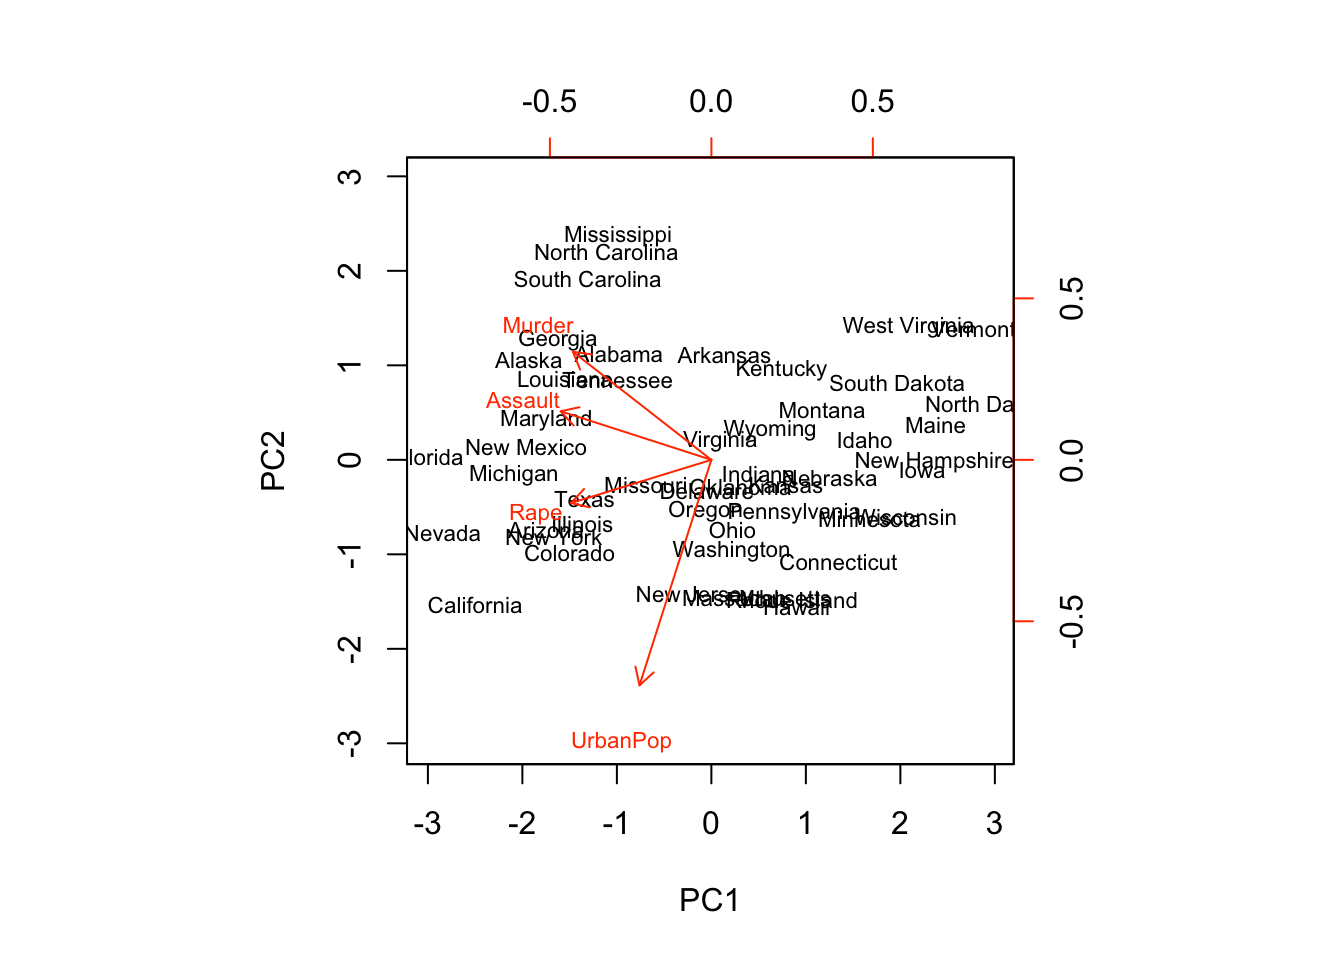
\includegraphics[width=0.7\linewidth]{USAarrests}
	\caption{\textbf{BiPlot}.
		Arrest type data for USA states. 
		Data includes urban population size, number of rape related arrests, assault related, and murder related ($p=4$). 
		Each city is presented against its two first PCs. 
		Arrows encode the loadings. 
		They show that PC1 encodes a general crime level, as it is the average of all type of crimes. 
		PC2 measures the level of urbanization, as it is dominated by the UrbanPopulation variable. 		
		\\ Source: \url{https://goo.gl/85qtKv}}
	\label{fig:usaarrests}
\end{figure}



\subsubsection{Scree Plot}
\label{sec:scree_plot}
[TODO]




\subsubsection{Why did Hotelling and Pearson arrive to the same solution?}
\label{sec:pca_intuition}

We have currently offered two motivations for PCA: 
(i) Find linear combinations $v_1,\dots,v_p$ that best distinguish between observations, i.e., maximize variance. 
(ii) Find the linear subspaces $\manifold_1,\dots,\manifold_p$ that best approximates the data.
The reason these two problems are equivalent, Pythagoras.

Informally speaking, the data has some total variance. 
In analogy to the $SST=SSR+SSE$ decomposition in linear regression, the total variance of $X$ can be decomposed into the part in $\manifold_q$, and the part orthogonal. 
The orthogonal part is the distance of $X$ from $\manifold_q$. 
Maximizing the variance in $\manifold_q$ is thus the same as minimizing the distance from $X$ to $\manifold_q$. 

The only unresolved matter- is why the solution to the variance maximization problem is a \emph{linear} subspace?
This is simply because all the scores, are linear combinations of columns of $X$, thus span a linear subspace, as is sought in the linear-subspace approximation view. 




\subsection{How many PCs can one recover?}
\label{sec:how-many-pcs}
On the face of it, with $p$ variables one can find $p$ PCs. 
Things are not that simple however.

In the population version of the problem, i.e., when $\Sigma$, and not $X'X$ is known, the number of PCs is the number of ``independent information pieces'' in $\x$. 
It will trivially be $p$ unless entries in $\x$ are fully multicollinear. 
Stating that $\Sigma$ has full rank, is thus identical to stating that the variables of $\x$ are not fully correlated, and thus, that $p$ PCs can be recovered. 

In the empirical version of the problem, i.e., when $X'X$, and not $\Sigma$ is known, things further complicate.
First, for purely algebraic reasons, there may be as many non zero eigenvalues as the rank of $X$.
Clearly, if $p>n$, variables of $X$ have to be linearly dependent, so that $X$, thus $X'X$, cannot possibly be of full rank.
Put differently, the number of PCs that may be computed is the same as the dimension of the rank of $X$. 

While the algebraic problem ends when $p<n$, the statistical one only begins, and ends if $n \gg p$. 
This is because $p$ eigenvalues and vectors include roughly $\bigO(p+p^2)$ parameters. 
If $p<n$ but $p\sim n$ then we do not have many observations per estimated parameter. 
In the statistical literature, this is known as a \emph{high-dimensional} problem. 
In the engineering parlance, we say we have low \emph{signal-to-noise}.
For a an analytical treatment of the statistical properties of PCA, see \cite{nadler2008finite}.
A purely algorithmic approach to the choice of $q$ is also available by adopting the supervised learning view of dimensionality reduction.
As can be seen from Eq.(\ref{eq:pca-dim-reduce}), PCA, like most other reduction approaches, is an Empirical Risk Minimization (ERM) problem.\marginnote{Empirical Risk Minimization}
As such, a resampling approach is made possible by putting data aside, and looking for a minimum of the out-of-sample reconstruction error\footnote{Using your favorite resampling algorithm such as V-fold CV, Bootstrapping, train-test, etc.}, as $q$ grows from $1$ to $p$. 


 


\subsection{PCA as a Graph Method}
\label{sec:pca_as_graph}

It turns out that we may find the sequence of best approximating linear subspaces, i.e., the PCs, without the actual measurements $X$, but only with a dissimilarity graph. 
In particular, with the $n\times n$ graph $\dissimilaritys$ of Euclidean distances between individuals: $\dissimilaritys_{i,j}:= \normII{x_i-x_j}$. 

It should come of no surprise that we don't need the actual measurements, $X$, since the optimal loadings, $v$, only depend on the covariance $\Sigma$, or its empirical counterpart, $X'X$. 
It may, however, be quite surprising that given only the distances between individuals, we may not recover the covariance between variables, $X'X$, but we can recover the PCs. 
Put differently, to find a low dimensional $\manifold$ that approximates the data, we don't need the whole data, but rather, only the graph of distances between data points. 

For proof of the above statement, we refer the reader to \citet[Sec.18.5.2]{friedman2001elements}

This observation will later be very useful for other dimensionality reduction algorithms, which operate not on the original data points, but rather, on dissimilarity graphs. 

\begin{think}
	Is it surprising that for a low dimensional representation of the data we only need to know the distances between points?
	Is it surprising that the PCs are agnostic to the means of the data?
\end{think}




\subsection{PCA as Supervised Linear Regression}
\label{sec:pca-as-supervised}
There is a strong link between dimensionality reduction and supervised learning.
Look at Eq.(\ref{eq:pca-dim-reduce}), does it not look very familiar to a linear regression?
Indeed, PCA can be thought of as finding a small set of predictors that linearly predict $X$. 
Almost all supervised learning algorithms can thus be applied to dimensionality reduction, by viewing $X$ as the labels, $y$, of some latent scores in $\manifold$.








\section{Preliminaries}

\subsection{Terminology}

\begin{tcolorbox}
	\begin{description}
		
		\item[Variable] \Aka \emph{dimension}, or \emph{feature} in the machine learning literature, or \emph{column} for reasons that will be obvious in the next item. 
		
		\item[Data] \Aka \emph{sample}, \emph{observations}. 
		Will typically consist of $n$, $p$ dimensional vectors.
		We typically denote the data as a $n\times p$ matrix $X$. 
		
		\item[Manifold] A space which is regular enough so that it is \emph{locally} has all the properties of a linear space. 
		We will denote an arbitrary manifold by $\manifold$, and by $\manifold_q$ a $q$ dimensional\footnote{You are probably used to thinking of the \emph{dimension} of linear spaces. We will not rigorously define what is the dimension of a manifold, but you may think of it as the number of free coordinates needed to navigate along the manifold.} manifold.
		
		
		\item[Embedding] Informally speaking: a ``shape preserving'' mapping of a space into another. 
		
		\item[Linear Embedding] An embedding done via a linear operation (thus representable by a matrix). 
		
		\item[Generative Model] Known to statisticians as the \emph{sampling distribution}. 
		The assumed stochastic process that generated the observed $X$. 
		
	\end{description}
\end{tcolorbox}




\subsection{Motivations for dimensionality reduction}

\begin{description}
	\item [Scoring] Give each observation an interpretable, simple score (Hotelling's motivation).

	\item [Latent structure] Recover unobservables from indirect measurements. 
	E.g: Blind signal reconstruction, CT scan, cryo-electron microscopy, etc. 
	
	\item [SNR] Denoise measurements before further processing like clustering, supervised learning, etc. 
	
	\item [Compression] Save on RAM ,CPU, and communication when operating on a lower dimensional representation of the data. 
	
\end{description}







\subsection{Properties of a dimensionality reduction approaches}
Here are some properties that characterize dimensionality reduction approaches. 
The reader is advised to try and characterize each approach along the following properties:
\begin{description}
	\item [Generative vs. algorithmic] Refers to the motivation of the approach. Is it stated as an algorithm, or stated via some generative probabilistic model. 
	PCA is purely algorithmic. 

	\item [Linear $\manifold$ vs. non-linear $\manifold$.]
	Is the target manifold linear or not?
	In PCA, $\manifold$ is linear.

	\item [Linear embedding vs. non-linear embedding.] 
	Is the embedding into $\manifold$ a linear operation?
	In PCA, the embedding is linear, and indeed, represented by a matrix. 
	
	\item [Learning an embedding vs. an embedding function?]
	Will we need to apply the reduction to new data? 
	If yes, we need to learn an \emph{embedding function}, $g:x \mapsto g(x)\in \manifold$.
	If no, and we merely want to low dimensional representation of existing data, $\set{g(x_i)}_{i=1}^n$, we only need to learn an embedding. 
	PCA learns an embedding \emph{function}.
	
	\item [Euclidean vs. non-Euclidean.] 
	Many dimensionality reduction methods only need a dissimilarity (i.e. distance) graph to operate. 
	The Euclidean distance is historically the most popular dissimilarity measure.
	Some approaches are agnostic to the measure used, some have Euclid hard-wired into them, and some, hard-wire themselves with some non-Euclidean norm. 
	PCA has Euclid hard-wired. 
\end{description}

\begin{remark}[Non linear manifolds and non-linear embeddings]
	The distinction we make between non-linear \emph{embeddings} and non-linear manifolds is non-standard in the literature. 
	The term \emph{non-linear space embedding} is used in both contexts, but typically only for the type of embedding, and not the target manifold.
\end{remark}


\subsection{Dimensionality Reduction and Supervised Learning}
\label{sec:dim-reduce-and-supervised}

In the machine learning literature, dimensionality reduction belongs in the \emph{unsupervised} type of learning. 
Indeed, class labels are not required to reduce dimension.
The problem, however, are not unrelated, as demonstrated for the PCA problem (Sec~\ref{sec:pca-as-supervised}), $X$ can be viewed as the labels, making dimensionality reduction a supervised learning problem, with \emph{unobservable}, or \emph{missing} features. 








\section{Latent Variable Generative Approaches}
All generative approaches to dimensionality reduction will include some unobserved set of variables, which we can try to recover from the observable $X$. 
The unobservable variables will typically have a lower dimension than the observables, thus, dimension is reduced. 
We start with the simplest case of linear Factor Analysis. 


\subsection{Factor Analysis (FA)}

FA originates from the psychometric literature. 
We thus revisit the IQ (actually g-factor) Example~\ref{ex:iq}:
\begin{example}[g-factor\footnote{\url{https://en.wikipedia.org/wiki/G_factor_(psychometrics)}}]
	
	Assume $n$ respondents answer $p$ quantitative questions: $x_i \in \reals^p, i=1,\dots,n$. 
	Also assume, their responses are some \emph{linear} function $\loadings \in \reals^p$ of a single personality attribute, $s_i$. 
	We can think of $s_i$ as the subject's ``intelligence''.
	We thus have 
	\begin{align}
	x_i = \loadings s_i + \varepsilon_i
	\end{align}
And in matrix notation, for $q<p$ latent attributes:
	\begin{align}
	\label{eq:factor}
		X = \latentn \loadings  +\varepsilon,
	\end{align}
where $\loadings$ is the $q \times p$ matrix of factor loadings, and $\latentn$ the $n \times q$ matrix of latent personality traits. 
In our particular example where $q=1$, the problem is to recover the unobservable intelligence scores, $s_1,\dots,s_n$, from the observed answers $X$.	
\end{example}


We may try to estimate $\latentn \loadings $ by assuming some distribution on $\latentn$ and $\varepsilon$ and apply maximum likelihood.
Under standard assumptions on the distribution of $\latentn$ and $\varepsilon$, recovering  $\latentn$ from $\estim{\latentn \loadings }$ is still impossible as there are infinitely many such solutions.
In the statistical parlance we say the problem is \emph{non identifiable}, and in the applied mathematics parlance we say the problem is \emph{ill posed}.
To see this, consider an orthogonal \emph{rotation} matrix $\rotation$ ($\rotation' \rotation=I$). For each such $\rotation$: $ \latentn \loadings = \latentn \rotation' \rotation \loadings = \latentn^* \loadings^* $.
While both solve Eq(\ref{eq:factor}), $\loadings$ and $\loadings^*$ may have very different interpretations. 
This is why many researchers find FA an unsatisfactory inference tool.


\begin{remark}[Identifiability in PCA]
	The non-uniqueness (non-identifiability) of the FA solution under variable rotation is never mentioned in the PCA context. Why is this?
	This is because the methods solve different problems. 
	The reason the solution to PCA is well defined is that PCA does not seek a single $\latentn$ but rather a \emph{sequence} of $\latentn$ with dimensions growing from $1$ to $p$. 
\end{remark}


\begin{remark}[Linear and non-linear embeddings]
	In classical FA in Eq.(\ref{eq:factor}) is clearly an embedding to a linear space. 
	The one spanned by $\latentn$. 
	Under the classical probabilistic assumptions on $\latentn$ and $\varepsilon$ the embedding itself is also linear, and is sometimes solved with PCA. 
	Being a generative model, there is no restriction for the embedding to be linear, and there certainly exists sets of assumptions for which the FA embedding is non linear. 
\end{remark}

\paragraph{FA Terminology}
The FA terminology is slightly different than PCA:
\begin{itemize}
	\item \textbf{Factors}: The unobserved attributes $\latentn$. 
	Not to be confused with the \emph{principal components} in the context of PCA.

	\item \textbf{Loadings}: 
	The $\loadings$ matrix; the contribution of each factor to the observed $X$.

	\item \textbf{Rotation}: An arbitrary orthogonal re-combination of the factors, $\latentn$, and loadings, $\loadings$, which changes the interpretation of the result.
\end{itemize}


The FA literature does offer several heuristics to ``fix'' the solution of the FA. 
These are known as \emph{rotations}:
\begin{itemize}
	\item \textbf{Varimax}: 
	By far the most popular rotation. Attempts to construct factors that are similar to the original variables, thus facilitating interpretation\footnote{This can be seen as a "soft" approach to sPCA (Sec.\ref{sec:sPCA})}.
	
	\item \textbf{Quartimax}: 
	Seeks a minimal number of factors to explain each variable. 
	May thus result factors that are uninterpretable, since they all rely on the same variables.
	
	\item \textbf{Equimax}: A compromise between Varimax and Quartimax. 
	
	\item \textbf{Oblimin}: 
	Relaxes the requirement of the factors to be uncorrelated, so that they may be similar to the original variables; even more so than in varimax. 
	This facilitates the interpretability of the factors. 
	
	\item \textbf{Promax}: 
	A computationally efficient approximation of oblimin.
\end{itemize}



\subsection{Non Linear Factor Analysis}
Classical FA deals with features, $X$, that are linear in the latent factors, $\latentn$. 
Like any other generative model approach, it can be easily extended to deal with non-linear functions of the latent factors: $X=g(S)$, provided that $g:\reals^q \mapsto \reals^p$ is one-to-one. 
This problem is a non-linear embedding into a linear space (the one spanned by $\latentn$).
It can also be seen as the generative counterpart of kPCA (Sec.\ref{sec:kpca}) or auto-encoders (Sec.\ref{sec:auto_encoders}).




\subsection{Independent Component Analysis (ICA)}
\label{sec:ica}


Like FA, ICA is a family of latent space models, thus, a \emph{meta-method}.
It assumes data is generated as some function of the latent variables $\latentn$. 
In many cases this function is assumed to be linear in $\latentn$ so that ICA is compared, if not confused, with PCA and even more so with FA. 

The fundamental idea of ICA is that $\latentn$ has a joint distribution of \emph{non-Gaussian independent} variables. 
This independence assumption, solves the the non-uniquness of $\latentn$ in FA.

Being a generative model, estimation of $\latentn$ can then be done using maximum likelihood, or other estimation principles. 

ICA is a popular technique in signal processing, where $\loadings$ is actually the signal, such as sound in Example~\ref{ex:blind-signal}.
Recovering $\loadings$ is thus recovering the original signals mixing in the recorded $X$. 



\begin{remark}[ICA and FA]
	The solutions to the (linear) ICA problem can ultimately be seen as a solution to the FA problem with a particular rotation $\rotation$ implied by the probabilistic assumptions on $\latentn$.
	Put differently, the formulation of the (linear) ICA problem, implies a unique rotation, which can be thought of as the rotation that returns components that are as far from Gaussian as possible. 
\end{remark}


\begin{remark}[Linear and non-linear embeddings]
	In classical ICA in Eq.(\ref{eq:factor}) is clearly an embedding to a linear space. 
	The one spanned by $\latentn$. 
	The probabilistic assumptions on $\latentn$ and $\varepsilon$ the embedding itself being non linear, thus solved as an optimization problem, and not via PCA. 
\end{remark}




%\subsubsection{Mathematics of ICA}
%For ease of presentation we present a simple setup, which can be considerably generalized. 
%In this setup, we will first analyze the population problem, i.e., in terms of random variables. 
%We thus replace the data $X$, with the random vector $\x$, and afterwards consider implementation for finite samples. 
%\begin{itemize}
%	\item $\x=\latentn \loadings $, implying that $\x$ is \emph{linear} in the latent components, and the latent space is of dimension $\rank=p$. 
%	It follows that $s=\loadings'X$.
%	\item $\x$ has been pre-whitented, so that $\cov{\x}=I$.
%	\item Distance between distributions are measured using the Kullback-Leibler divergence (KL): $\kl{\x}{\latentn}$.
%\end{itemize}
%
%The optimization problem in this simple ICA is to find an orthogonal matrix $\loadings$, for which:
%(i) the components of $\loadings'\x$ are independent;
%(ii) $\loadings'\x$ is a good approximation of $\x$.
%Formally: 
%\begin{align}
%\label{eq:ica_optimization}
%\argmin{\loadings \text{ orthogonal} \;; \loadings'\x \text{ independent}}{\kl{\loadings'\x}{\x}}.
%\end{align}
%
%
%By enforcing the independence constraint in Eq.(\ref{eq:ica_optimization}), and due to the properties of the KL divergence, Eq.(\ref{eq:ica_optimization}) is equivalent to
%\begin{align}
%\label{eq:ica_optimization2}
%\argmin{\loadings \text{ orthogonal}}{\sum_{j=1}^{\rank} \entropy(\loadings_j\x)- \entropy(\x)}
%\end{align}
%where $\entropy(\x)$ denotes the Entropy of the random variable $\x$ (Definition \ref{def:entropy}).
%Now, $\entropy(\x)$ is obviously fixed, so we need to minimize $\entropy(\loadings_j\x)$. 
%A classical result in information theory, is that the Gaussian distribution has the maximal entropy. 
%Minimizing $\entropy(\loadings_j\x)$ can thus be interpreted as finding a matrix $\loadings$ such that its columns return random variables, $\loadings_j\x$, that are as \emph{non-Gaussian} as possible.
%
%This is where the population analysis ends. 
%The insight we take from it, is that finding independent components, is actually finding non-Gaussian combinations of $\x$. 
%The different implementations of ICA, indeed look for a matrix $\loadings$ which returns the most non-Gaussian combinations of the observed $X$. 
%
%














\section{Purely Algorithmic Approaches}

We now discuss dimensionality reduction approaches that are not stated via their generative model, but rather, directly as an algorithm.
This does not mean that they cannot be cast via their generative model, but rather they were not motivated as such.



\subsection{Multidimensional Scaling (MDS)}
\label{sec:mds}

Very roughly speaking, MDS can be thought of as a variation on PCA, that (i) begins with a distance graph\footnote{The term Graph is typically used in this context instead of Network. But a graph allows only yes/no relations, while a network, which is a weighted graph, allows a continuous measure of similarity (or dissimilarity). It is thus more appropriate.} $\dissimilaritys$, and (ii) embeds into a two-dimensional space.
Regarding (i), we have already seen in Section~\ref{sec:pca_as_graph} that PCA really only needs a similarity graph, $X'X$, and not the whole $X$.  
Regarding (ii), the embedding into two dimensions is motivated by that fact that MDS is typically used for visualization. 

MDS aims at embedding a graph of distances, while preserving the original distances.
Basic results in graph/network theory \citep[e.g.][]{graham1988isometric} suggest that the geometry of a graph cannot be preserved when embedding it into lower dimensions. 
The different types of MDSs, such as \emph{Classical MDS}, and \emph{Sammon Mappings}, differ in the \emph{stress function} penalizing for geometric distortion.

Sadly, MDS may scale poorly to large dissimilarity matrices, and the optimization may converge to a local minimum.
The solution to MDS is an embedding and not an embedding \emph{function}. 
When new data points are made available, the embedding will thus have to be re-learned.





\subsubsection{Mathematics of MDS}
We start with either a dissimilarity network $\dissimilaritys=(\dissimilarity_{i,j})$, or a similarity network $\similaritys=(\similarity_{i,j})$.
Similarities can be thought of as correlations, and dissimilarities as distances (which are indeed the typical measures in use).
Define $z_i \in \reals^\rank$ the location of point $i$ in the target linear space of rank $\rank$. 
The $z_i$'s are set to minimize some penalty for geometric deformation called the \emph{stress function}.
Typical stress functions include:
\begin{description}
	
	\item[Classical MDS] \Aka \emph{Torgerson scaling} begins with the empirical covariance as the similarity measure,$\similarity_{i,j}:= \scalar{x_i-\bar x}{x_j-\bar{x}}$, and minimizes the squared average distortion:
	\begin{align}
	\label{eq:mds_classical}
	\argmin{z_1,\dots,z_n}{\sum_{i,j=1}^{n} (\similarity_{i,j}-\scalar{z_i-\bar z}{z_j-\bar{z}} )^2}.
	\end{align}
	
	\item[Least Squares] \Aka \emph{Kruskal-Shepard} starts with a Euclidean distance graph,$\dissimilarity_{i,j}= \normII{x_i-x_j}$, and minimizes the squared average distortion. 
	\begin{align}
	\label{eq:mds_stress}
	\argmin{z_1,\dots,z_n}{\sum_{i \neq j} (\dissimilarity_{i,j}-\norm{z_i-z_j} )^2}.
	\end{align}
	
	\item[Sammon Mapping] Also known as \emph{Sammon's stress}, starts with a Euclidean distance graph and aims at minimizing the average \emph{proportion} of distortion:
	\begin{align}
	\label{eq:mds_sammon}
	\argmin{z_1,\dots,z_n}{\sum_{i \neq j} \frac{(\dissimilarity_{i,j}-\norm{z_i-z_j} )^2}{\dissimilarity_{i,j}}}.
	\end{align}
	
\end{description}




\begin{remark}[MDS and PCA]
	MDS with ``classical scaling'' (\aka Torgerson scaling) returns the exact same embedding as PCA with $2$ PCs.
\end{remark}


\begin{remark}[MDS and Graph Drawing]
	If the purposes of lowering the dimension is visualization, then the dimension of $\manifold$ will typically be $2$. 
	Embedding in $2$ dimensional linear spaces is of great interest for visualization, and indeed there is a whole field called \emph{Graph Drawing}\footnote{\url{https://en.wikipedia.org/wiki/Graph_drawing}}, which focuses on these problems.
	For instance, the very popular \emph{force embedding}\footnote{\url{https://en.wikipedia.org/wiki/Force-directed_graph_drawing}} in the D3 java-script libraries stems from the Graph Drawing literature. 
\end{remark}



\subsubsection{Non-Metric MDS}
The above approaches to MDS start with the actual distances between points. 
If the actual distances are replaced with some monotonic function of these, then it is only the \emph{ordering} of distances that drives the solution.
This is known as \emph{non-metric MDS}.





\subsection{Local MDS}
\label{sec:localMDS}

\begin{example}[Non-Euclidean surface]
\label{ex:non-euclidean}
	Consider data of coordinates on the globe. 
	At short distances, constructing a dissimilarity graph with Euclidean distances will capture the true distance between points. 
	At long distances, however, the Euclidean distances as grossly inappropriate. 
	A more extreme example is coordinates on the brain's cerebral cortex.
	Being a highly folded surface, the Euclidean distance between points is far from the true geodesic distances along the cortex's surface\footnote{Then again, it is possible that the true distances are the white matter fibers connecting going within the cortex, in which case, Euclidean distances are more appropriate than geodesic distances. We put that aside for now.}.
\end{example}

Local MDS is aimed at solving the case where we don't know how to properly measure distances. 
It is an algorithm that compounds both the construction of the dissimilarity graph, and the embedding. 
The solution of local MDS, as the name suggests, rests on the computation of \emph{local} distances, where the Euclidean assumption may still be plausible, and then aggregate many such local distances, before calling upon regular MDS for the embedding.

Because local MDS ends with a regular MDS, it can be seen as a non-linear embedding into a linear $\manifold$. 





\subsection{Isometric Feature Mapping (Isomap)}
\label{sec:isomap}

Isomap, also known as \emph{Principal Coordinate Analysis}, operates very similarly to local MDS, but with a different algorithm to compute the dissimilarity matrix.



\subsection{Kernel Principal Component Analysis (kPCA)}
\label{sec:kpca}

Back to the height-weight problem in Example\ref{ex:bmi}: assume we want to construct a ``bigness'' score, that best separates between individuals, but we no longer constrain it to be a linear function of the height and weight.
Adopting the variance maximization view of PCA, we could try to find the best separating score $g(x)$ by solving 
\begin{align}
\label{eq:kpca_wrong}
	\argmax{g}{\cov{g(\x)}}
\end{align}
where $g(x):\reals^p \mapsto \reals^q$, maps an individual's $p$ features to a $q$ dimensional score in $\manifold$.

Without any constraints on $\manifold$, thus on $g$, we will overfit \andor not be able to compute $g$ as optimization is done in a infinite dimensional space. 
We thus have two matters to attend:
(i) We need to constrain $g(x)$.
(ii) We need the problem to be computable.
This is precisely the goal of kPCA. 

If we choose the right $g$'s, the solution of Eq.(\ref{eq:kpca_wrong}) may take a very simple form. 
The classes of such $g$'s are known as Reproducing Kernel Hilbert Spaces (RKHS). 
At an intuitive level, RKHS's are subspaces of ``the space of all functions'', which:
(i) Are defined via a \emph{kernel function} we need to specify. Each kernel defines a different subspace. 
(ii) They have a very particular structure so that the optimal $g$ is not linear in $X$, but is linear in some simple and known transformation of $X$-- the kernel. 



\begin{remark}[kPCA and Manifold learning]
	kPCA is seen by some as the ``father'' of all manifold learning algorithms. 
	Algorithms such as IsoMap, LLE, LaplacianEigenmaps, were motivated as generalizations of kPCA.
\end{remark}



\paragraph{Mathematics of kPCA}
[TODO]





\subsection{Local Linear Embedding (LLE)}
\label{sec:lle}

LLE is similar in spirit to Isomap and LocalMDS.
It differs, however, in the way similarities are computed, and in the way embeddings are performed. 
Unlike localMDS, which computes local distances and ends with a \emph{global embedding}, LLE computes local distances and performs \emph{local linear embeddings}.
The resulting approximating manifold $\manifold$, being the ``stitching'' of many linear spaces, is ultimately non linear.



\subsection{Laplacian Eigenmaps}
Just like LLE, Laplacian Eigenmaps is an algorithm to measure distances and embed local neighborhoods of the original $X$ space.


\subsection{Maximum Variance Unfolding}
A different solution to the same problem a LLE.



\subsection{Self Organizing Maps (SOM)}
SOMs are special in our context in that the target $\manifold$, is not a bona-fide manifold. 
SOMs are typically designed for visualization, so they embed into a $2$ dimensional space. 
The target space, $\manifold$, is a \emph{polygon mesh}.
Polygon meshes are easy to compute with, but hard to analyze mathematically. 
In particular, the ``stitching'' between polygons is a very irregular structure that does not satisfy the definition of a \emph{manifold}.



\subsection{Principal Curves and Surfaces}
The algorithm iterates until it returns a curve of a surface.
In the curve case, it will return a curve with the \emph{self consistency} property. 
I.e., a curve with a path that is the average of all it's closest data points.\marginnote{Self Consisntecy}
Roughly speaking, one can think of this as a generalization of k-means from points to curves. 
Each such curve smoothly connects the k-means cluster centres.
Using the same, slightly inaccurate depiction, a \emph{principal surface} is manifold with dimension greater than $1$, connecting these k-means cluster centres.
In both cases, the output is a continuous parametrization of the curve or the surface.

It is highly uncommon to approximate the data with manifolds with a dimension larger than $2$, as typically the method is used for projecting the data before visualizing \andor clustering.





\subsection{Auto Encoders}
\label{sec:auto_encoders}

To present \emph{auto-encoders}, \aka \emph{auto-associator} or \emph{Diabolo network}, we restate the PCA space embedding formulation of Eq.(\ref{eq:pca-dim-reduce}):
\begin{align}
	\argmin{\loadings\in \reals^{q \times p}, S\in \reals^{n \times q}}{\normF{X- \latentn \loadings}}
\end{align}
because of the invariance of the solution to rotations, and at the cost of interpretation, we may freely assume that $\loadings \loadings'=I$.
If $q=p$ then at the optimum $X=\latentn \loadings$ so that $\latentn=\loadings' X$. We thus have:
\begin{align}
	\argmin{\loadings\in \reals^{q \times p}}{\normF{X- X\loadings'\loadings}}.
\end{align}

This formulation of PCA problem, allows us to see that the single layer \emph{auto-encodres}, assumes that $X$ is some non-linear $g:\reals^p \mapsto \reals^p$ of scores with loadings $W$:
\begin{align}
	\argmin{W\in \reals^{q\times p}}{\normF{X- g(XW')W}}.
\end{align}
For the right choice of $g$, autoencoding can be understood as a \emph{neural network} used to predict $X$ latent scores (see Sec~\ref{sec:dim-reduce-and-supervised}).
Alternatively, as a purely-algorithmic counterpart fo non-linear FA and ICA.







\subsection{Matrix Factorization}
\label{sec:matrix_factorization}
[TODO]



\subsection{Information Bottleneck}
[TODO]

%The \emph{information bottleneck} is an information theoretic framework, due to \cite{tishby_information_1999}, that generalizes the idea of dimensionality reduction and data compression.
%It is a general statement of the problem of maximal compression of $X$, while preserving as much of the information in $X$ as possible.
%To state the general problem we require some definitions from information theory.
%
%\begin{definition}[Entropy]
%The entropy of a random variable $\x$ is defined as the expected negative log density of $\x$: 
%$$\expect{-\log \pdf(\x)}.$$
%\end{definition}
%
%\begin{definition}[Mutual Information]
%The mutual information between two random variable $\x$ and $\y$ is defined as : 
%$$\expect{\log \frac{\pdf(\x,\y)}{\pdf(\x) \pdf(\y)}}.$$
%\end{definition}
%
%Informally speaking, the entropy is a measure of the variability of a distribution, and the mutual information is a measure of deviation from independence, i.e., captures the amount of information $\x$ carries on $\y$, and vice-versa.
%With this intuition, and denoting the compression of $x$ by $y=g(x)$, we may define the compression problem as:
%\begin{align}
%	\argmin{g}{arg2}
%\end{align}


\begin{remark}[Information Bottleneck and ICA]
	[TODO]
\end{remark}




\subsection{Bibliographic notes}
To read more on almost anything, see \citet{friedman2001elements}.
For a detailed review of ICA see \cite{hyvarinen2000independent}. 
For more on MDS \cite{borg2005modern}.
For manifold learning see \citet{mohri2012foundations}.








\section{Dealing with the high-dimension}

As we previously mentioned (Sec.\ref{sec:how-many-pcs}), it is hard to accurately estimates directions of co-variability with little data. 
For some intuition, think of recovering a ``bigness score'' (Example~\ref{ex:bmi}) from only 3 individuals ($p=2,n=3$). 
Would you trust the recovered index?

In high dimensional problems, \aka low signal-to-noise regimes, we will introduce some regularization, to reduce variance, as the cost of some bias. 
For generative models, regularization can always be introduced with Bayesian priors, say, some matrix-valued distribution as a prior on $\loadings$. 
For purely algorithmic approaches (such as PCA), regularization has to be be hard-wired into the algorithm.





\subsection{Simplified Component Technique LASSO (SCoTLASS)}

SCoTLASS can be thought of as PCA, where sparse $\loadings$ are preferred as solutions.
By ``sparse'' we mean that $\loadings$ has many zero entries. 
We favor sparse solutions both to deal with the very low SNR of high dimensional problems, but also for better interpretation.

\begin{think}
	Why is it easier to interpret the PCs when $\loadings$ has many zero entries?
\end{think}

The mathematics of SCoTLASS looks like the variance maximization formulation of PCA with an equality and an inequality constraint.
\begin{align}
\label{eq:scotlass}
	\argmax{v}{v'(X'X)v  + \lambda \normI{v} \text{ such that } \normII{v}=1 }
\end{align}
Sadly, Eq.(\ref{eq:scotlass}) is hard to solve numerically.


\subsection{Sparse Principal Component Analysis (sPCA)}
\label{sec:sPCA}

Starting from the linear-space approximation view of PCA (not variance maximization), and with the numerical difficulties of SCoTLASS, we define the sPCA problem:
\begin{align}
\label{eq:spca}
	\argmin{\loadings,\theta}{\normF{X-\Theta \loadings X} + \lambda_2 \normII{\loadings} + \lambda_1 \normI{\loadings} \text{ such that } \normII{\Theta}=1},
\end{align}
where $\loadings$ is the matrix of all loadings, $\normF{.}$ the Frobenius matrix-norm, $\normII{.}$ the $l_2$ matrix-norm, and $\normI{.}$ the $l_1$ matrix-norm.

sPCA can be seen as the SCoTLASS problem, where $\normII{\loadings}=1$ is relaxed to $ \normII{\loadings}\leq t$ for ease of computation.
It can also be seen as a particular type of rotation, since just like the FA problem, when $p>n$ then PCA is also non-identifiable. 





\subsection{Sparse kernel principal component analysis}
If you liked the idea of sparse loadings (for interpretability, or SNR), and you liked the idea of embedding the data into non-linear, infinite dimensional RKHS, why not marry the ideas?
See \citet{tipping2001sparse}.



\subsection{Random Projections}
You feel that the data is SOOOOO large that you don't have time to find embeddings that are optimal in any sense. 
You thus want to reduce the dimension of the data and don't care how good it is. 
How about simply multiplying $X$ by a \emph{random} matrix, projecting from $\reals^p$ to $\reals^q$, for $q<p$.
It turns out, that this is not a bad strategy!
Look for the Johnson-Lindenstrauss lemma, for example in \citet{mohri2012foundations}.


\newpage
\bibliographystyle{abbrvnat}
\bibliography{dim_reduce.bib}



\end{document}
